\documentclass[10pt]{beamer}
%\documentclass[handout,10pt]{beamer}
%\mode<presentation>
%{
%  \usetheme{Berkeley}
%  \usecolortheme{seahorse}
%  \usefonttheme{default}
%  \setbeamertemplate{navigation symbols}{}
%  \setbeamertemplate{caption}[numbered]
%}

\usetheme{metropolis}

\usepackage[english]{babel}
\usepackage[utf8x]{inputenc}
\usepackage{caption}
\usepackage{multirow}
\usepackage{mathrsfs}
\usepackage{graphicx}
\usepackage{amsmath}
\usepackage{graphicx}
\usepackage[compatibility=false]{caption}
\usepackage{subcaption}
\usepackage[normalem]{ulem}
\DeclareMathOperator{\tr}{tr}
\usepackage{textpos}
\usepackage{animate}

\title[FMSP Further Mathematics]{Graphing Functions}
%\titlegraphic{\includegraphics[height=1.57cm]{logo.jpg}}
\author[Scott Morgan]{\textbf{Scott Morgan}}
\institute{\textit{Further Mathematics Support Programme - WJEC A-Level Further Mathematics} \\
\textit{13th January 2018}
\\ \\ \\
\textit{scott3142.com | @Scott3142}}
\date

\begin{document}

\begin{frame}
  \maketitle
\end{frame}

\begin{frame}{Graph Sketching - Asymptotes}
  \begin{itemize}[<+->]
    \item [\textbf{Step 1.}] Find any points at which the graph cuts the coordinate axes.
    \item [\textbf{Step 2.}] Find any stationary points where $f'(x) = 0$.
    \item [\textbf{Step 3.}] Find any vertical asymptotes (denominator zero?)
    \item [\textbf{Step 4.}] Consider the behaviour of the graph for numerically large x, giving the equation of any horizontal or oblique asymptotes.
    \item [\textbf{Step 5.}] Complete the sketch.
  \end{itemize}
\end{frame}

\begin{frame}{Graph Sketching - Asymptotes}
  \begin{itemize}[<+->]
    \item [\textbf{Step 4.}] Consider the behaviour of the graph for numerically large x, giving the equation of any horizontal or oblique asymptotes.
    \vspace{3mm}
    \item If the degree of the denominator is greater than the degree of the numerator, then $y\to 0$ as $x\to\pm\infty$. This means that there is a horizontal asymptote at $y = 0$.
    \begin{itemize}
      \item
        \begin{equation}
          f(x) = \frac{1}{x}
        \end{equation}
      \item
        \begin{equation}
          f(x) = \frac{x}{x^2 + 2}
        \end{equation}
      \item
        \begin{equation}
          f(x) = \frac{1}{x(x^2 + 1)}
        \end{equation}
      \item
        \begin{equation}
          f(x) = \frac{5-3x}{(x-1)(x-3)}
        \end{equation}
      \item
        \begin{equation}
          f(x) = \frac{x}{(x-1)^2}
        \end{equation}
    \end{itemize}
  \end{itemize}
\end{frame}

\begin{frame}{Graph Sketching - Asymptotes}
  \begin{itemize}
    \item <1-> [\textbf{Step 4.}] Consider the behaviour of the graph for numerically large x, giving the equation of any horizontal or oblique asymptotes.
    \vspace{3mm}
    \item <1-> If the degree of the denominator is equal to the degree of the numerator, then there is a horizontal asymptote other than the $x$-axis. You can find this asymptote by dividing out.
    \begin{itemize}
      \item <2->
        \begin{align*}
          f(x) &= \frac{(x+1)^2}{(x-1)(x-2)} \only<3->{\textcolor{red}{ = 1 - \frac{4}{x-1} + \frac{9}{x-2}}} \\
          \only<4->{&\textcolor{blue}{\implies \text{Horizontal asymptote at $y=1$}}}
        \end{align*}
      \item <5->
        \begin{align*}
          f(x) &= \frac{5-3x}{x-3} \only<6->{\textcolor{red}{ = -3 - \frac{4}{x-3}}}
          \\
          \only<7->{&\textcolor{blue}{\implies \text{Horizontal asymptote at $y=-3$}}}
        \end{align*}
    \end{itemize}
  \end{itemize}
\end{frame}

\begin{frame}{Graph Sketching - Asymptotes}
  \begin{columns}
    \begin{column}{0.5\textwidth}
      \begin{center}
        \begin{figure}[h!]
          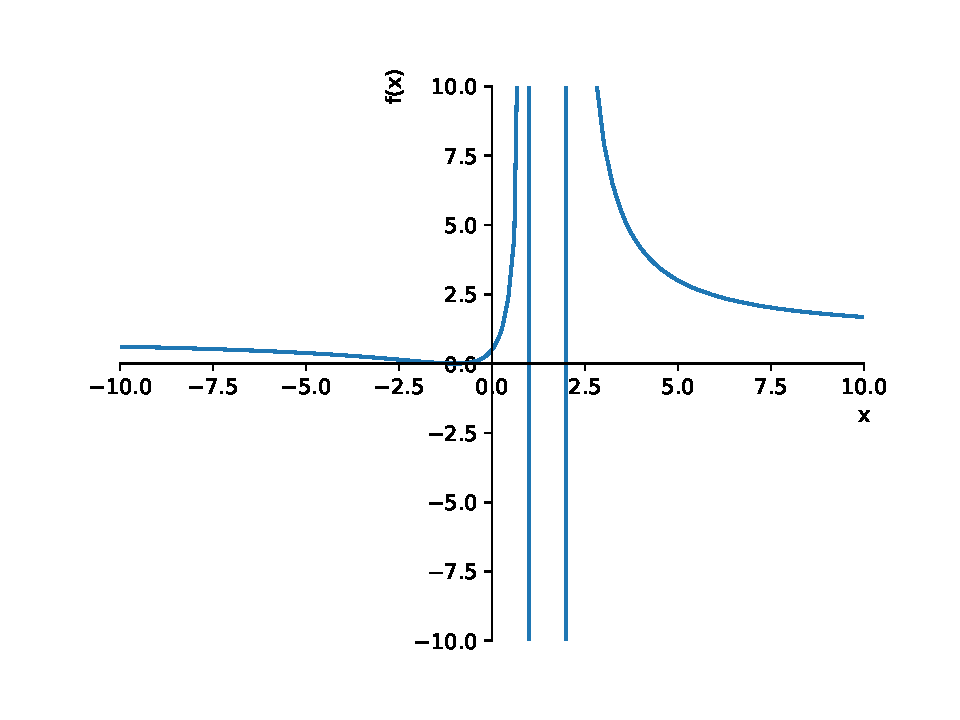
\includegraphics[width=\textwidth]{beamer-pics/asymptote-1.pdf}
          \caption*{$y = 1 - \frac{4}{x-1} + \frac{9}{x-2}$}
        \end{figure}
      \end{center}
    \end{column}

    \begin{column}{0.5\textwidth}
      \begin{center}
        \begin{figure}
          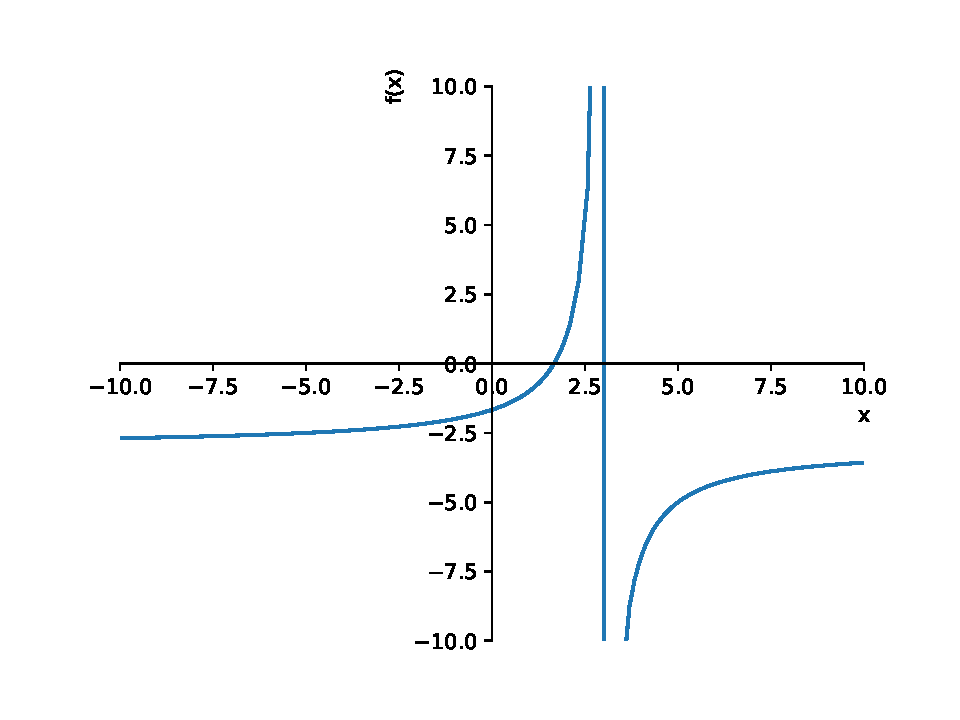
\includegraphics[width=\textwidth]{beamer-pics/asymptote-2.pdf}
          \caption*{$y = -3 - \frac{4}{x-3}$}
        \end{figure}
      \end{center}
    \end{column}
  \end{columns}
\end{frame}

\begin{frame}{Graph Sketching - Asymptotes}
  \begin{itemize}
    \item <1-> [\textbf{Step 4.}] Consider the behaviour of the graph for numerically large x, giving the equation of any horizontal or oblique asymptotes.
    \vspace{3mm}
    \item <1-> If the degree of the denominator is one less than the degree of the numerator, then there is an oblique asymptote. You can find this asymptote by dividing out.
    \begin{itemize}
      \item <2->
        \begin{align*}
          f(x) &= \frac{x^2+4}{x} \only<3->{\textcolor{red}{ = x + \frac{4}{x}}}
          \\
          \only<4->{&\textcolor{blue}{ \implies \text{Oblique asymptote is $y=x$}}}
        \end{align*}
      \item <5->
        \begin{align*}
          f(x) &= \frac{x(x+3)}{x-1} \only<6->{\textcolor{red}{ = x + 4 + \frac{4}{x-1}}}
          \\
          \only<7->{&\textcolor{blue}{ \implies \text{Oblique asymptote is $y=x+4$}}}
        \end{align*}
    \end{itemize}
  \end{itemize}
\end{frame}

\begin{frame}{Graph Sketching - Asymptotes}
  \begin{columns}
    \begin{column}{0.5\textwidth}
      \begin{center}
        \begin{figure}
          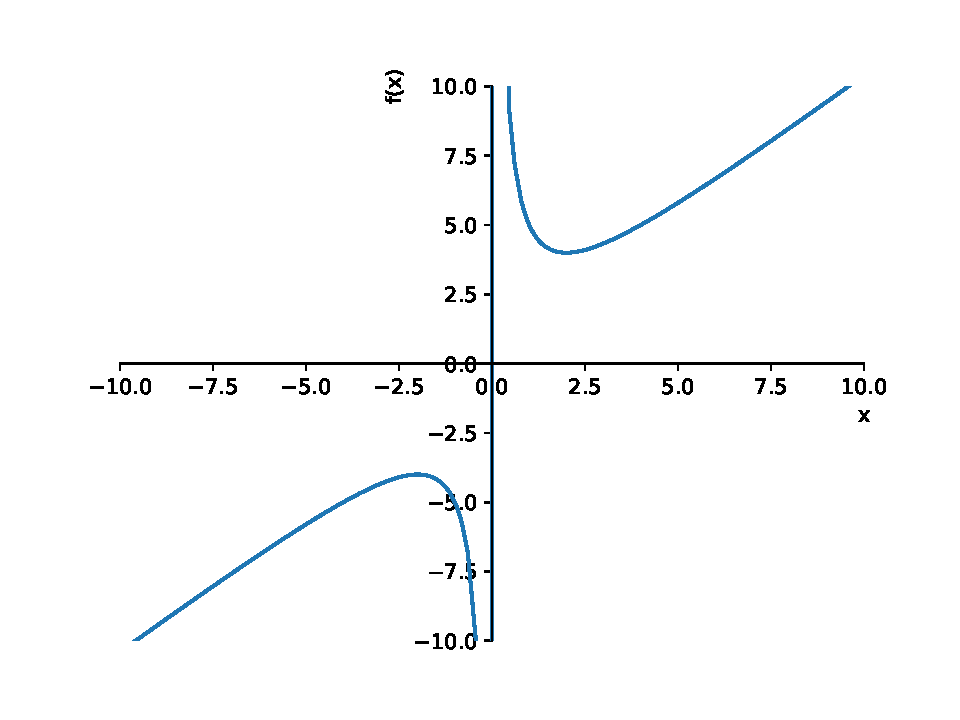
\includegraphics[width=\textwidth]{beamer-pics/asymptote-3.pdf}
          \caption*{$y = x + \frac{4}{x}$}
        \end{figure}
      \end{center}
    \end{column}

    \begin{column}{0.5\textwidth}
      \begin{center}
        \begin{figure}
          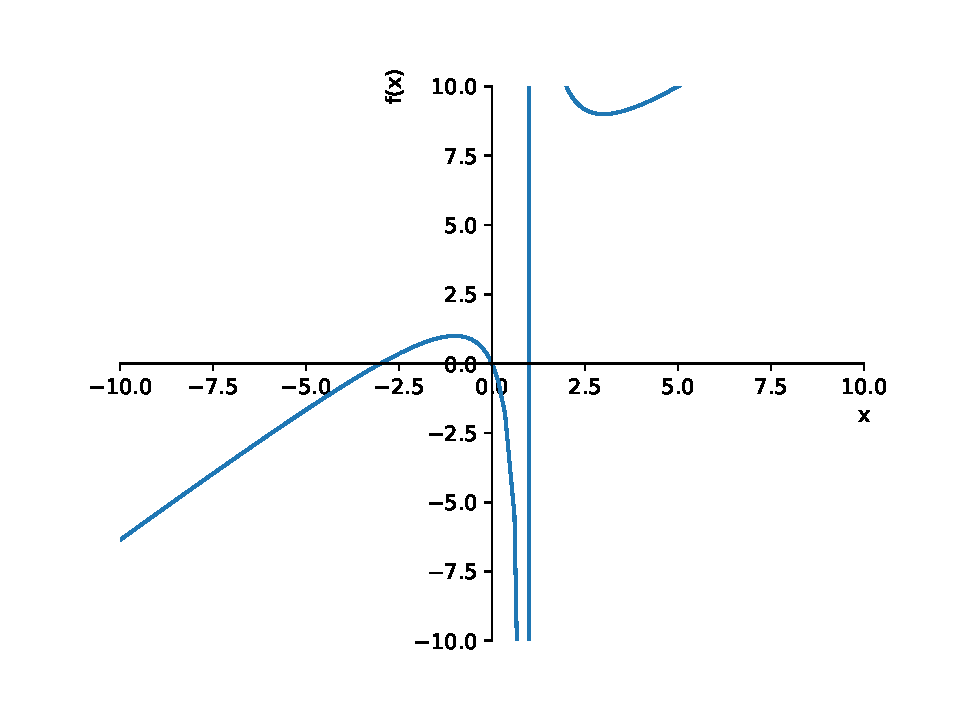
\includegraphics[width=\textwidth]{beamer-pics/asymptote-4.pdf}
          \caption*{$y = x + 4 + \frac{4}{x-1}$}
        \end{figure}
      \end{center}
    \end{column}
  \end{columns}
\end{frame}

\begin{frame}{Things to Remember}
  \begin{itemize}[<+->]
    \item Points at which the graph cuts the coordinate axes.
    \item Stationary points where $f'(x) = 0$.
    \item Vertical asymptotes (may be more than one!)
    \item Horizontal and oblique asymptotes.
  \end{itemize}
\end{frame}

\begin{frame}{Stationary Points}
  \begin{itemize}[<+->]
    \item We know that stationary points occur when $f'(x) = 0$.
    \item But how do we know if these points local maxima/minima?
  \end{itemize}

  \begin{columns}
    \begin{column}{0.5\textwidth}
      \only<3->{
        \begin{figure}
          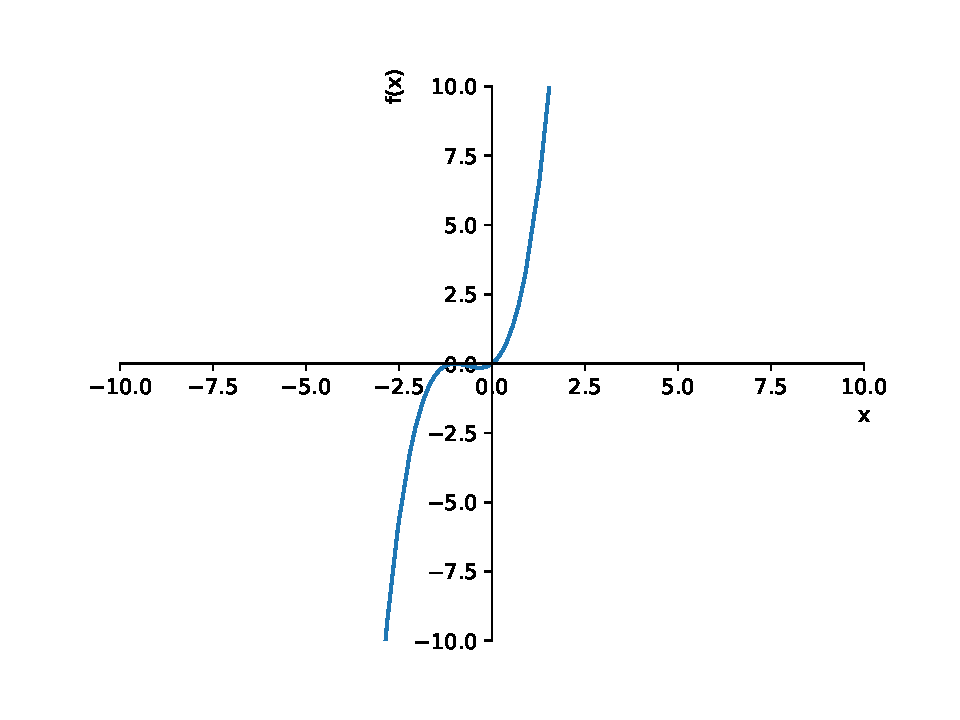
\includegraphics[width=\textwidth]{beamer-pics/asymptote-5.pdf}
          \caption*{$f(x) = x^3+2x^2+x$}
        \end{figure}
      }
    \end{column}

    \begin{column}{0.5\textwidth}
      \only<4->{
        \textbf{Second derivative test:}
        \begin{itemize}
          \item <5-> If $f''(x) < 0$, the stationary point at $x$ is concave down; \textbf{a maximum}.
          \item <6-> If $f''(x) > 0$, the stationary point at $x$ is concave up; \textbf{a minimum}.
        \end{itemize}
      }
    \end{column}
  \end{columns}
\end{frame}

\begin{frame}{Other Properties of Graphs - Odd \& Even}
  \begin{itemize}[<+->]
    \item An \textbf{even} function is one such that
      \begin{equation}
        f(x) = f(-x)
      \end{equation}
    \item An \textbf{odd} function is one such that
      \begin{equation}
        f(x) = -f(-x)
      \end{equation}
    \item Can you think of any examples of odd and even functions?
  \end{itemize}
\end{frame}

\begin{frame}{Other Properties of Graphs - Odd \& Even}
  \begin{columns}
    \begin{column}{0.5\textwidth}
      \begin{figure}
        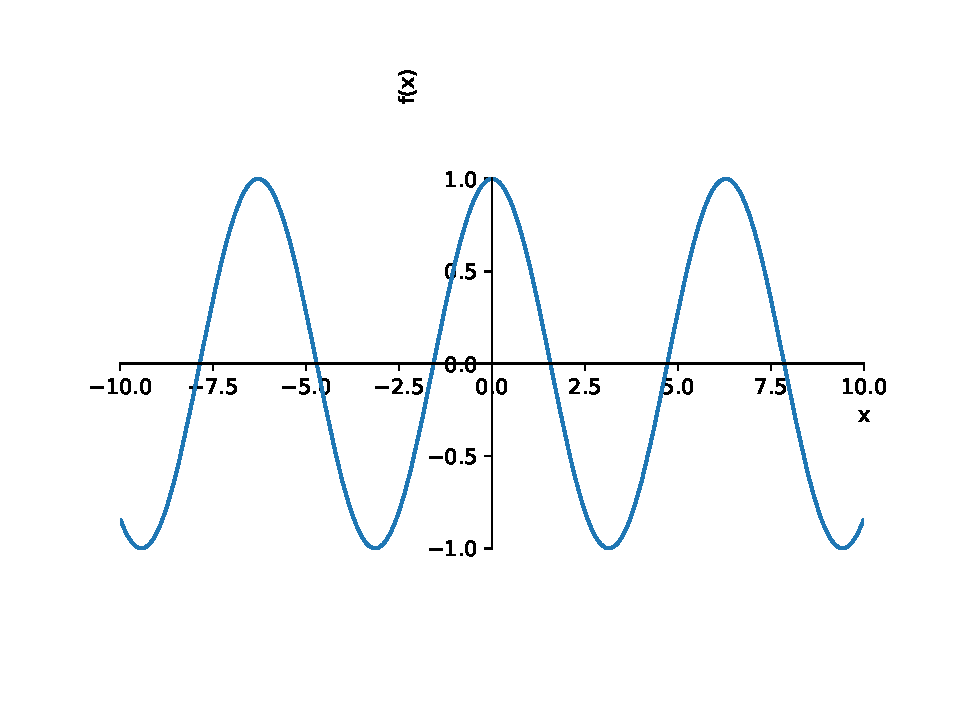
\includegraphics[width=\textwidth]{beamer-pics/even.pdf}
        \caption*{$f(x) = cos(x)$}
      \end{figure}
    \end{column}

    \begin{column}{0.5\textwidth}
      \begin{figure}
        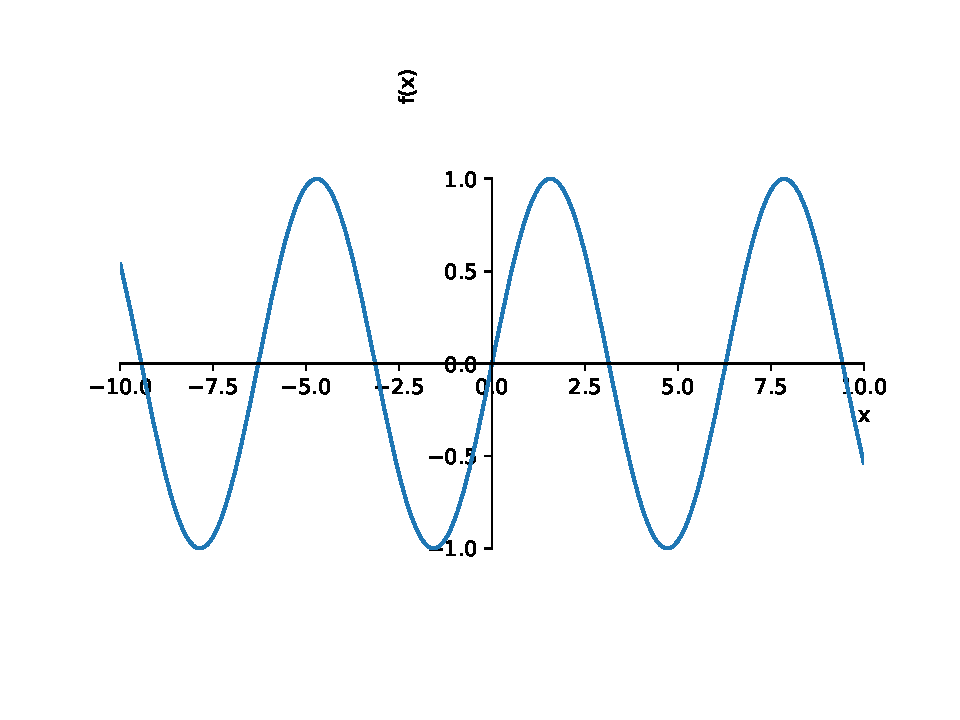
\includegraphics[width=\textwidth]{beamer-pics/odd.pdf}
        \caption*{$f(x) = sin(x)$}
      \end{figure}
    \end{column}
  \end{columns}
\end{frame}

\begin{frame}{Other Properties of Graphs - Image and Inverse Image}
  \begin{itemize}[<+->]
    \item The \textbf{image} of a set under a function is the set of values which that function maps the element of the set to. Consider
      \begin{equation}
        f(x) = x^2 + x + 1 \hspace{5mm} \text{for} \hspace{3mm} x \in [-2,1]
      \end{equation}
  \end{itemize}

  \begin{columns}
    \begin{column}{0.5\textwidth}
      \only <2->{
        \begin{figure}
          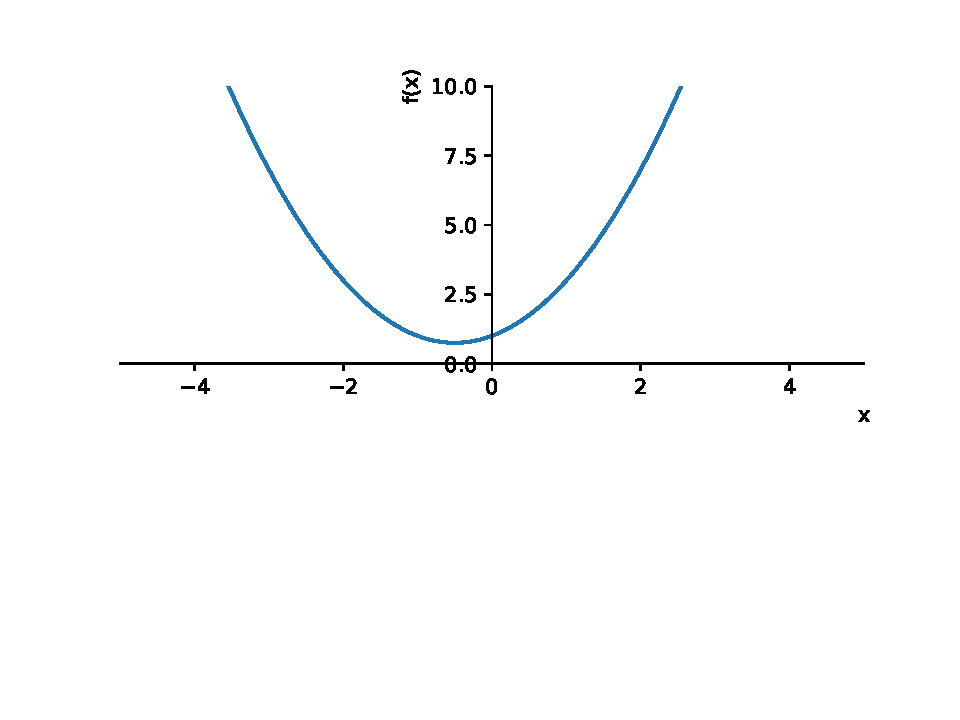
\includegraphics[width=\textwidth]{beamer-pics/image.pdf}
          \caption*{$f(x) = x^2 + x + 1$}
        \end{figure}
      }
    \end{column}

    \begin{column}{0.5\textwidth}
      \begin{itemize}
        \item <3-> The \textbf{image} of the set $[-2,1]$ is the part of the $y$-axis enclosed by the function in this $x$-range.
        \item <4-> In this case, $f([-2,1]) = \left[\frac{3}{4},3\right]$
      \end{itemize}
    \end{column}
  \end{columns}
\end{frame}

\end{document}
